\section{Protocol layers}
\textbf{Application}: works with messages. Is where applications and their protocols exist. Examples include HTTP, SMTP, FTP, and DNS.\\
\textbf{Transport}: works with segments. Transports application layer messages between specific applications on different hosts. Examples include TCP and UDP.\\
\textbf{Network}: works with datagrams. Transports segments from one host to another. Examples include IP and ICMP.\\
\textbf{Link}: works with frames. Transports datagrams between neighbouring network elements. Examples include Ethernet and WiFi.\\
\textbf{Physical}: works with bits. The physical medium connecting neighbouring network elements. Examples include copper cable, fibre optics, and radio waves.

\subsection{Application layer}
An application is identified by a 32 bit \textbf{IP address} and 16-bit \textbf{port number}. The IP address identifies the host, and the port number identifies the application on that host.

\subsubsection{The Web and HTTP}
\textbf{HTTP} is a stateless protocol which determines how web clients (such as browsers) interact with web servers. HTTP uses TCP, and either establishes one persistent session across many requests, which removes the expensive setup time for each request, or establishes a new session for each request, which prevents the client and server from needing to store information about a session that is not currently in use. When non-persistent sessions are used, each request takes approximately $2\cdot\text{round trip time}+\text{file transmission time}$, while with persistent sessions once a connection is established, each request takes approximately $\text{round trip time}+\text{file transmission time}$.\\
An \textbf{HTTP request} has this format:\\
\begin{verbatim}
GET /somedir/page.html HTTP/1.1
Host: www.someschool.edu
Connection: close
User-agent: Mozilla/5.0
Accept-language: fr
\end{verbatim}
Common request methods are: \textbf{GET} (request an object from the server), \textbf{POST} (send some data and the server should reply with a response object), \textbf{HEAD} (request an object, but the server only responds with the HTTP header, used for debugging), \textbf{PUT} (upload an object), \textbf{DELETE} (delete an object from the server). \textbf{GET} can also send data to the server, by appending queries to the URL, e.g. \verb|somesite.com/search?search=a+search+string|.\\
An \textbf{HTTP response} has this format:\\
\begin{verbatim}
HTTP/1.1 200 OK
Connection: close
Date: Tue, 18 Aug 2015 15:44:04 GMT
Server: Apache/2.2.3 (CentOS)
Last-Modified: Tue, 18 Aug 2015 15:11:03 GMT
Content-Length: 6821
Content-Type: text/html
data goes here
\end{verbatim}
Common response codes are: \textbf{200 OK} (request succeeded), \textbf{301 Moved Permanently} (requested object has been moved, the client will automatically request the new URL), \textbf{400 Bad Request} (message not understood by server), \textbf{404 Not Found} (requested document not found), \textbf{505 HTTP Version Not Supported} (server does not support the HTTP protocol version used in the request).\\
Sessions can be tracked using \textbf{cookies} by setting the \textbf{Set-Cookie} header in the response, and the client will send the cookie back in the request. Cookies can be used to store session information, user preferences, and shopping cart contents, or they can be IDs that are used to index a cookie database on the server.\\
\textbf{HTTP/2} is a new version of HTTP that is binary instead of textual, fully multiplexed, uses one connection for parallelism, uses header compression, and allows servers to push responses proactively into client caches.
\textbf{Web caches} satisfy HTTP requests on behalf of a server. A browser must be configured to request from a cache, and then if the page is already in the cache it can respond faster than the server could have. Web caches use conditional GETs to check if the page has been updated since the last time it was cached, by setting the \verb|If-Modified-Since| header line.\\

\subsubsection{Email and SMTP}
Email systems consist of user agents, mail servers, and the simple mail transfer protocol (STMP). When an email is sent, the user agent sends the email to the user's mail server, which then sends the email to the recipient's mail server, which then stores the email until the recipient's user agent requests it. STMP uses TCP with persistent connections, and pushes the email to the recipient's mail server, unlike HTTP which pulls objects from a server. An email header looks like this:
\begin{verbatim}
From: alice@aServer.com
To: bob@anotherServer.com
Subject: Hello
\end{verbatim}
\textbf{POP3} is a protocol used by the recipient's mail client to retrieve the email from the server. A user logs in with \verb|user <username>| and \verb|pass <password>|, then can list emails with \verb|list|, retrieve an email with \verb|retr|, and delete an email with \verb|dele|. Once the user has finished, all their actions are applied at the same time with \verb|quit|.\\
\textbf{IMAP} is a protocol used by the recipient's mail client to retrieve the email from the server. It is more powerful than POP3, as it allows the user to create, delete, and rename mailboxes, and allows the user to search for emails.\\
Today, most email clients are sent using a web browser, so emails are requested from servers using HTTP.

\subsubsection{DNS}
The \textbf{Domain Name System} is responsible for translating application layer hostnames to network layer IP addresses. It is a distributed database implemented in a hierarchy of DNS servers. When a request is made, the DNS client calls a local DNS server, which then calls a root DNS server, which then calls a top-level domain DNS server, which then calls an authoritative DNS server. The authoritative DNS server then sends the IP address back to the client. The local server will cache the IP address of the response, but will also cache the addresses of the various servers, meaning that the root servers are very rarely contacted. DNS resolution uses both recursive requests (the client asks the server to resolve the request) and iterative requests (the client asks the server to tell it the next server to contact). A hostname may map to many IP addresses, in which case the server responds with them in a random order. As the client usually picks the first one, this acts as a simple load balancing system.\\
A DNS request has this format:
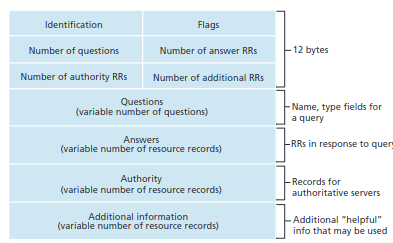
\includegraphics[width=\linewidth]{../images/w3n7dnsMessage.png}\\
And a record has the format \verb|<name, value, type, ttl>|. The \textbf{type} states what the record is, \verb|A| means \verb|name| is a hostname and \verb|value| is the corresponding IP address, \verb|NS| means \verb|name| is a domain and \verb|value| is the server knows the next step in resolving that domain, \verb|CNAME| means \verb|name| is an alias for \verb|value|, \verb|MX| means \verb|name| is a domain and \verb|value| is the mail server for that domain. The \textbf{TTL} is the time the record can be cached for.\\

\subsubsection{P2P and BitTorrent}
\textbf{Peer-to-peer} applications communicate directly with other peers without requiring a central server. P2P applications are used for file distribution, streaming, and telephony, as they are well suited to sharing large files.\\
If we have a system with $N$ hosts wishing to download an $F$ bit file, peer[$i$] having an upload rate of $u_i$ and a download rate of $d_i$, along with a server with an upload rate of $u_s$, then for a client server architecture the time for all clients to download the file is bounded by
\[
	D_{CS}\ge\max\left\{\frac{NF}{u_s},\frac{F}{d_{\min}}\right\}
\]
In a P2P system, each peer who gets a part of the file can distribute it onwards, and the download time is bounded by
\[
	D_{P2P}\ge\max\left\{\frac{F}{u_s},\frac{F}{d_{\min}},\frac{NF}{u_s+\sum^N_{i=1}u_i}\right\}
\]
$D_{P2P}$ equals that only when the server sends bits one at a time to each client.\\
\textbf{BitTorrent} is a popular P2P file distribution protocol. A file is broken into chunks, typically 256 KB each, and all peers for a file form a torrent. Each torrent has a tracker, which keeps a list of all active peers. When a new peer (we'll call Alice) joins a torrent, it contacts the tracker, which selects a random subset of peers and sends their IPs to Alice who attempts to open concurrent TCP connections with all the IPs it received. Each successful connection is counted as a "neighbouring peer", and over time some of those peers will leave while others join and establish connections, leading to Alice's neighbouring peers fluctuating over time. Every neighbour will have a different subset of chunks of the file, so Alice will periodically request a list of the chunks each of its neighbours has. Alice then determines which chunks are held by fewest of her neighbours and requests them first (rarest-first), this means that each chunk of a file should end up roughly equally distributed.\\
Alice will also receive requests for chunks for each of her neighbours, and she selects the four that are sending her the highest rate of bits, and reciprocates by sending them their requested chunks - these neighbours are known as \textbf{unchoked}. She recalculates the top four every 10 seconds. Every 30 seconds, she also selects one random neighbour (in this case Bob) and sends it chunks - this neighbour is \textbf{optimistically unchoked}. If Alice makes it into Bob's top four uploaders and he will reciprocate, and may also make it into Alice's top four. This means that peers will gradually match up with other peers that are capable of uploading at comparable rates, and that a new peer will get chunks that it can trade with its neighbours. All other neighbouring peers receive nothing from Alice, and are \textbf{choked}.

\subsubsection{QUIC}
QUIC is an application layer protocol built on top of UDP, and provides error and congestion control, along with security. Integrating all of these allow it to set up reliability and authentication in 1 RTT, instead of requiring 2 RTTs that are required for TCP + TLS. In addition, QUIC can multiplex multiple streams over a single connection.

\subsection{Transport layer}
\textbf{Multiplexing} is the process of taking data from multiple applications and sending it over a single link. UDP uses a tuple of \verb|(destination IP, destination port)| to identify which application the data is for, while TCP uses a tuple of \verb|(source IP, source port, destination IP,| \verb|destination port)|.

\subsubsection{UDP}
\textbf{User Datagram Protocol} is a connectionless protocol that simply packages a bytestream into segments and sends it to the destination. It provides no guarantees of delivery, order, or duplicate packets. It performs simple error checking, and is used for applications that can tolerate some loss, such as streaming media, DNS, and SNMP. A UDP segment has this format:\\
\begin{center}
	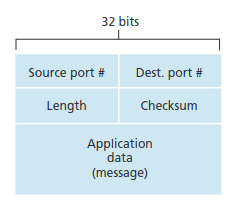
\includegraphics[width=0.7\linewidth]{../images/w4n3udpSegment.png}\\
\end{center}

\subsubsection{TCP}
\textbf{Transmission Control Protocol} provides a delivery service that guarantees that a byte stream sent using it will arrive in order with no duplicate packets. It is a \textbf{connection oriented service}, meaning that the client and server exchange transport layer level control information before the application layer messages start to flow. TCP creates a segment up to the \textbf{maximum segment size (MSS)} which is determined so that the TCP segment when encapsulated in an IP datagram can fit within the largest link-layer frame that can be sent by the sending host. Ethernet has a \textbf{maximum transmission unit (MTU)} of 1500 bytes, and the TCP+IP headers are usually 40 bytes, so the MSS is typically 1460 bytes. A TCP segment has this format:\\
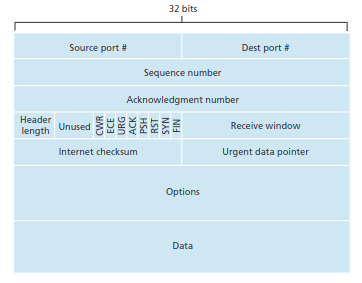
\includegraphics[width=\linewidth]{../images/w5n2tcpSegmentStructure.png}\\
The \textbf{receive window} is the amount of data that the receiver is willing to accept, and is used to prevent the sender from overwhelming the receiver. The \textbf{options field} is usually empty, but can be used to negotiate a window scaling factor for high speed use cases or for timestamping. The 4 bit \textbf{header length} is the length of the header in 32 bit words, usually when there are no options it is 5. The flags CWR and ECE are for congestion notification, \textbf{URG} is used if there is an urgent pointer in the \textbf{urgent data pointer} field, though this is rarely used, \textbf{ACK} is set if the segment is an acknowledgement for a successfully received segment, \textbf{PSH} is used to push data to the application layer immediately, again rarely used, \textbf{RST} is used to reset the connection, \textbf{SYN} is used to establish a connection, and \textbf{FIN} is used to terminate a connection.\\
\textbf{Sequence and acknowledgement numbers}: TCP uses cumulative acknowledgement, so the acknowledgement number is the next byte the receiver expects to receive. The sequence number is the byte number of the first byte in the segment. TCP usually, but isn't required to, cache data that is received after a gap in the sequence numbers, and only deliver it to the application layer once the gap is filled.\\
\textbf{Retransmission timers}: TCP uses a retransmission timer with a variable timeout period. The period is calculated using a sample RTT based off of one currently transmitted but not yet ACKed segment, resulting in a new value approximately once every RTT. This is used to calculate an estimated RTT, using an \textbf{exponential weighted moving average (EWMA)} using the following formula:
\[
	\begin{aligned}
		\text{EstimatedRTT}  =  (1- & \alpha)\cdot\text{EstimatedRTT} \\
		+                           & \alpha\cdot\text{SampleRTT}
	\end{aligned}
\]
The recommended, but not required, value for $\alpha$ is $0.125$.
The variability of the sample RTT is also calculated, using:
\[
	\begin{aligned}
		\text{DevRTT}=(1- & \beta)\cdot\text{DevRTT}                                            \\
		+                 & \beta\cdot\left\vert\text{SampleRTT}-\text{EstimatedRTT}\right\vert
	\end{aligned}
\]
If there is little variation of sample RTT values, then $\text{DevRTT}$ will be small, while if there is a lot of variability it will be large.
The recommended value of $\beta$ is $0.25$.

The timeout value is then set using both these values:
\[
	\text{TimeoutInterval}=\text{EstimatedRTT}+4\cdot\text{DevRTT}
\]
This means that the timeout stays close to the estimated RTT, but if $\text{DevRTT}$ grows then so does the timeout period.
An initial $\text{TimeoutInterval}$ of 1 second is recommended, and if a timeout occurs then the timeout is doubled until a segment is received, after which the timeout is recalculated using the above equation.\\
\textbf{Flow control} prevents the sender from overflowing the receive buffer of the receiver. The receiver advertises a \textbf{receive window} in each segment, which is the amount of data it is willing to accept. Each time the receiver sends a segment, it includes the current amount of space it has in its receive buffer. The sender uses this value to ensure that the number of unacknowledged bytes in transit is never more than the receive window, ensuring that the receiving buffer never overflows. In the case that the receiver's buffer is full, and it gives the sender a window size of 0, and the receiver has no segments it wants to send, the sender will continue to send 1 data byte segments to the receiver until the receiving application starts reading from the buffer again and the recipient will start responding with non-zero window sizes.\\
\textbf{Connection setup}: The \textbf{three-way handshake} is used to establish a connection. The client sends a segment with the SYN flag set and a randomly chosen initial client sequence number \verb|client_isn| to the server, this is the SYN message. The server responds with a segment with the SYN and ACK bits set, a random initial server sequence number \verb|server_isn|, and the acknowledgement number set to \verb|client_isn+1|, this is the SYN-ACK message. The client then sends a segment with the ACK bit set, the sequence number set to \verb|client_isn+1|, and the acknowledgement number set to \verb|server_isn+1|, this is the ACK message. The connection is now established, and data transfer can begin.\\
\textbf{Connection teardown}: either party can end the connection at any point by sending a segment with the FIN bit set. The other party responds with an ACK, then its own FIN, which the first party responds to with an ACK. The connection is now closed.\\
\textbf{Congestion control}: TCP performs congestion control by maintaining a congestion window \verb|cwnd| alongside the receive window \verb|rwnd| ant the maximum amount of data in flight at any time is \verb|min(cwnd, rwnd)|. A \textbf{loss event} occurs when either a timeout occurs or 3 duplicate ACKs are received. If \verb|rwnd| is large enough it can be ignored, so we will focus only on \verb|cwnd|.\\
The TCP congestion control algorithm consists of 3 parts:\\
1. \textbf{Slow start}: initially, TCP ramps up \verb|cwnd|, starting from 1 MSS, and increases it by 1 MSS every time an ACK is received. If a loss event occurs, \verb|cwnd| is set back to 1 MSS and the process repeats, except TCP also maintains a variable \verb|ssthresh| (slow-start threshold), which is set to half the \verb|cwnd| value at the time the loss event occurred. Once \verb|cwnd| reaches \verb|ssthresh|, slow start ends and enters congestion avoidance mode.\\
2. \textbf{Congestion avoidance}: now, \verb|cwnd| is around half the value at which congestion last occurred, so TCP must be more careful. Therefore, \verb|cwnd| is increased by 1 MSS every RTT, usually by increasing the window by $MSS/\text{number of bytes in flight}$ for each ACK. If a timeout occurs, the response is the same as in slow start, \verb|ssthresh| is set to half of \verb|cwnd|, \verb|cwnd| is set to 1 MSS, and slow start mode is reentered. If 3 duplicate ACKs are received, then \verb|ssthresh| is set to \verb|cwnd|, and \verb|cwnd| is halved (+ 3 MSS for the duplicate ACKs received), and it enters fast recovery mode.\\
3. \textbf{Fast recovery}: in this mode, \verb|cwnd| is increased by 1 MSS for every duplicate ACK received for the missing segment that caused fast recovery to start. Once that segment is ACKed, TCP returns to congestion avoidance with \verb|cwnd| set to \verb|ssthresh|, returning to the state it was in.\\
The state machine for TCP congestion control is as follows:
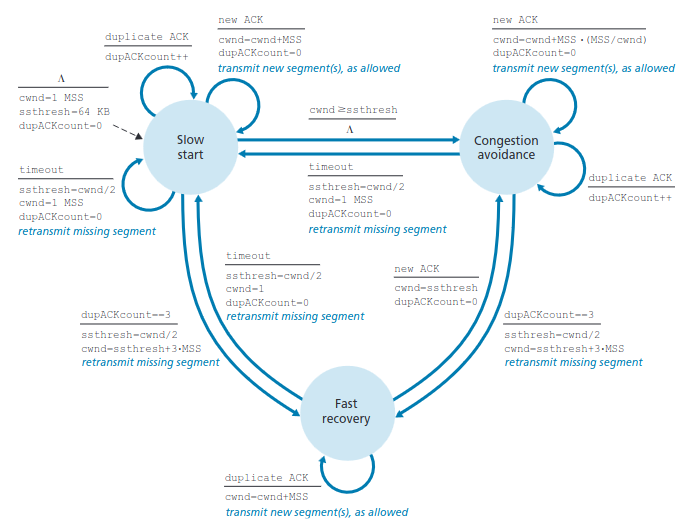
\includegraphics[width=\linewidth]{../images/w5n4tcpCongestionFsm.png}\\
TCP uses \textbf{additive increase, multiplicative decrease (AIMD)} for congestion control.\\
If a router is experiencing congestion, it may set the ECN bit in TCP ACKs passing through it, which causes the receiver to halve its \verb|cwnd|.\\
\textbf{TCP throughput}: if $w$ is the window size, and when a loss event occurs the window halves to get $W$, then the throughput of a TCP connection is given by:
\[
	\text{Average throughput of a connection}=\frac{0.75\cdot W}{RTT}
\]
\textbf{Fairness}: if multiple TCP connections pass through the same bottleneck link, they tend to share the bandwidth fairly if they both have the same RTT. If they don't the connection with the smallest RTT will claim a larger portion of the available connection. This is the mechanism by which it converges on fairness:
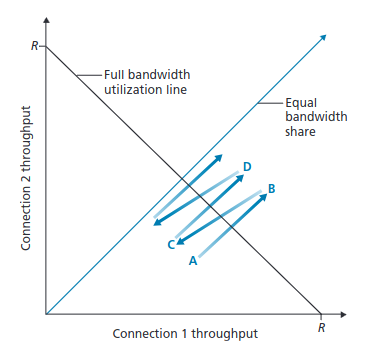
\includegraphics[width=\linewidth]{../images/w5n4tcpFairness.png}\\

\subsection{Network layer}
The network layer routes packets between hosts. It runs on every host and router on a network. The network layer consists of two components: the \textbf{control plane} determines the best routes across the network, and the \textbf{data plane} forwards packets based on those routes. The internet's network layer is the \textbf{Internet Protocol (IP)}, which provides only a "best effort service", with no guarantees of packets being delivered.\\

\subsubsection{IPv4}
The \textbf{IPv4} header has this format:
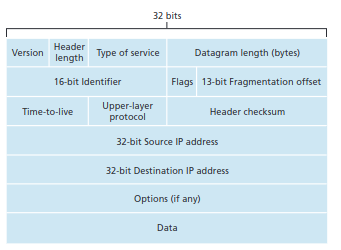
\includegraphics[width=\linewidth]{../images/w7n3ipv4Datagram.png}\\
The minimum header length is 20 bytes, but it may be longer if there are options set. \textbf{TTL} is the number of hops until the datagram gets dropped. This is decremented each time a router processes it, preventing a datagram circulating endlessly. \textbf{Protocol} is the transport layer protocol that the datagram is carrying, with 6 being TCP, 17 being UDP, and 1 being ICMP. If a datagram travels across a physical link with a smaller MTU than the datagram, it will be fragmented. The \textbf{fragment offset} is the offset of the fragment in the original datagram, and the \textbf{identifier} is the same for all fragments of a datagram. The \textbf{header checksum} is calculated over the header only, and is recalculated at each router due to the TTL changing. \textbf{type-of-service bits} allow different types of IP datagrams to be distinguished from each other. This is also where the ECN bits are set\\
\textbf{Addressing}: every interface between a physical link and a host/router has a 32 bit \textbf{IP address}, which is unique across the entire internet. This allows for only around 4 billion IP addresses, so routers use \textbf{network address translation (NAT)} to allow multiple devices to share a single IP address by having the router present itself to the outside network as though it is only one device, and each request being sent from a device within the internal network gets assigned an arbitrary port and its sender address changed to be the router's address. When responses arrive, the router uses the destination port to map that message to an internal IP, and sends the packet on to there. A device behind a NAT router will have an internal IP of 10.0.0.x, which is a reserved IP block for internal addresses. A network is divided into \textbf{subnets} by dividing it along each router. Every interface in the same subnet has the same subnet mask (prefix), e.g. \verb|223.1.1.0/24|, which means that the first 24 bits are the same for all IPs in that subnet. This means that an external router will only need to consider what subnet a packet needs to be routed to, while an internal router only needs to look at the last bits of the IP address.\\
\textbf{DHCP} is a method to automatically assign IP addresses to devices on a network. The DHCP address assignment protocol occurs in four steps: 1. \textbf{DHCP server discovery}: when a new host connects, it first must find a DHCP server. It does this by sending a UDP packet to port 67 of the IP broadcast address (255.255.255.255), and sets the source address to 0.0.0.0. 2. \textbf{DHCP server offer(s)}: when a DHCP server receives a packet on port 67, it then responds with an offer of an IP address, network mask, and a duration for that IP address to remain valid, again sent to the broadcast address this time on port 68. 3. \textbf{DHCP request}: the client selects one of the offered IP addresses, and responds to the broadcast address with that IP, as well as echoing back the configuration parameters 4. \textbf{DHCP ACK}: the server responds with an ACK message confirming the parameters.\\

\subsubsection{IPv6}
An \textbf{IPv6} header has this format:
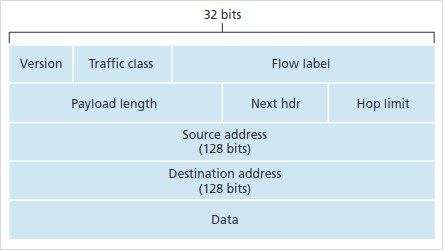
\includegraphics[width=\linewidth]{../images/w7n4ipv6Format.png}\\
IPv6 uses 128 bit addresses, which allow for $2^{128}$ addresses. The header is fixed to always be 40 bytes long, so we only need to provide the \textbf{payload length}. IPv6 packets cannot be fragmented, instead if an overly large datagram arrives at a router, it drops it and sends a "Packet Too Big" ICMP message back to the sender. There also no checksum, which is left to the link and transport layer protocols. Instead of an options field, the \textbf{next header} field can be set to an options field, which contains options then itself states the contained protocol. IPv6 datagrams can be tunnelled through IPv4 if a router doesn't support IPv6, by encapsulating the IPv6 datagram in an IPv4 datagram.\\

\subsubsection{Data plane}
A router consists of:\\
\textbf{Input ports}: physically terminates the incoming physical link, a queue of messages waiting to be routed, and finally performs the lookup to determine where the packet should be routed to.
\textbf{Switch fabric}: connects all input ports to all output ports, and is used to move a datagram from an input to an output.
\textbf{Output ports}: contains a queue of messages waiting to be transmitted, and the physical transmitter used to send messages onto the next physical link. (Note that sometimes there will be an input and an output port on a physical link, if the physical link supports 2 way communication).
A \textbf{routing processor}: performs control plane functions such as maintaining the routing tables.\\
When a packet arrives at the router, the router table finds the longest matching prefix in the routing table and applies that behaviour to the packet. Packets are switched using one of several approaches:\\
\textbf{Switching via memory}: the oldest approach. The router is simply a computer, and when a packet arrives it triggers an interrupt, then the routing processor copies the packet to memory, determines how to route that packet, then copies it back out to the output buffer. In this scenario, if the processor has a bandwidth of $B$ bps, then the overall throughput must be less than $B/2$. In addition, only one packet can be routed at a time, as only one memory read or write can occur over the shared system bus. \textbf{Switching via a bus}: here, the input port prepends an internal routing label to the packet indicating the correct output link. This is then written to a bus connecting all inputs to all outputs, and only the indicated output stores the packet. Here, the switching speed of the router is limited by the bus speed. \textbf{Switching via an interconnection network}: by connecting a network of busses with toggleable connections at each intersection multiple packets can be routed in parallel. In the example below, a packet arriving at $B$ or $C$ could be simultaneously routed to outputs $X$ or $Z$, alongside the current $A\rightarrow Y$ routing occurring.\\

\subsubsection{Control plane}
The control plane determines how packets are routed across the network. There are two approaches: \textbf{per router control}: a routing algorithm runs on every router, and so routers talk to each other to determine what the best routes are, and \textbf{logically centralised control}: a single routing controller determines the best routes, and tells all routers on the network what their forwarding tables should be.\\
\textbf{Routing algorithms} determine "good" paths from senders to receivers for some definition of "good", generally the shortest or fastest path. Routing algorithms can be \textbf{static} if routes are computed once and rarely change, or \textbf{dynamic} if routes are recomputed as the network changes. They are \textbf{load sensistive} if they dynamically vary the routes based on the current network load.\\
A \textbf{link-state algorithm} has every router send a message to every other router with the state of its links, and then each router constructs a graph of the network and uses Dijkstra's algorithm to find the shortest path. Each router should advertise its link costs at random intervals to prevent route oscillations. The \textbf{distance-vector (DV) algorithm} is iterative, asynchronous, and distributed, and scales better than link state as routers only need to send messages to their neighbours. Each router maintains a distance vector, which is the cost of the shortest path to every other router. The router then sends its distance vector to its neighbours, who then update their distance vectors based on the received vectors. Distance vectors are updated by finding the minimum cost to each destination, based on which neighbour has the lowest cost from the current router to that one added to the cost from that router to the destination based on the received distance vector. The \textbf{Bellman-Ford equation} is used to update the distance vector, and is:
\[
	d_x(y)=\text{min}_v\{c(x,v)+d_v(y)\}
\]
It is possible for loops to form if link costs increase, where one node $x$ routes through $y$ to get to $z$, while $y$ routes through $x$ to get to $z$. In the above case, when $c(x,y)$ goes up to 60, then $y$ recalculates its shortest path to 6, but this is based on $z$ saying it has a $c(z,x)=5$ path available. $z$ then gets this update, and recalculates $c(z,x)$ to 7, and so on until the costs have counted up to be more than 50 (44 iterations). This is known as the \textbf{count-to-infinity problem}. This can be partially fixed by having $z$ lie to $y$ and say it has no route to $x$ because its route to $x$ goes via $y$ (the \textbf{poisoned reverse}). This is not perfect though, as larger loops can still form.\\
DV and LS algorithms differ on a number of key metrics: \textbf{Message complexity}: LS requires each node to be sent the cost of every link in the network, or $O(|N|+|E|)$ messages, and when a link cost changes this must all be sent again. DV only sends messages between neighbours at each iteration, and these messages need only to be sent after a link cost changes, significantly reducing the number of messages needed. \textbf{Speed of convergence}: LS takes $O(|N|^2)$ to calculate all routes, while DV converges slowly and can have routing loops until the network converges. \textbf{Robustness}: single corrupt routers can influence DV more significantly, as every router depends on every other routers' communication, causing incorrect values to diffuse through the whole network.\\

\subsubsection{Large scale routing}
Routers are organised into \textbf{autonomous systems (ASes)}, with every router within an AS running the same routing algorithm, and one global routing protocol managing all inter-autonomous system routing.\\
\textbf{Open shortest path first (OSPF)} is an intra-AS routing algorithm which uses link-state information flooding and Dijkstra's algorithm. Individual link costs must be configured by the system administrator, giving them control over the routed flows. Advantages include: \textbf{security}: link state updates may be authenticated, ensuring that only trusted routers can participate in the OSPF protocol. \textbf{Multiple same-cost paths}: when multiple paths to a destination have the same cost, then both may be used. \textbf{Hierarchy within ASes}: an OSPF AS can be broken down into smaller hierarchical areas, with each running its own OSPF link-state algorithm.\\
The internet's inter-AS routing system is the \textbf{border gateway protocol (BGP)}. BGP uses routing tables in the format \verb|(x,I)|, where \verb|x| is a prefix and \verb|I| is one of the router's interfaces. BGP determines prefix reachability by having each router broadcast all the prefixes that are reachable from itself, and the path from it to those prefixes. Using this example network:
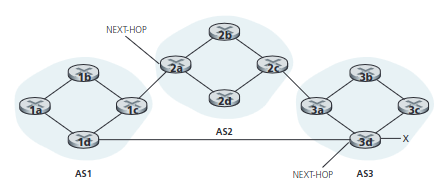
\includegraphics[width=\linewidth]{../images/w9n2bgpExampleNetwork.png}\\
Router \verb|3a| would send an \textbf{external BGP (eBGP)} message to \verb|2c| saying \verb|AS3 x| (to reach subnet \verb|x| go via \verb|AS3|). \verb|2c| would then send \textbf{internal BGP (iBGP)} messages to all the other routers in \verb|AS2| to tell them to go via \verb|AS3|. \verb|2a| would then send a eBGP message to \verb|1c|, which would tell its AS there is a path to subnet \verb|x| along \verb|AS2 AS3 x|. In addition, there would be a path \verb|AS3 x| from \verb|1d|. If there are multiple shortest paths, then the route is filtered by a manually set local preference, then the shortest AS path, then the closest exit point (\textbf{hot potato routing}).\\
Routing policy may be set so that an AS won't transport packets that came from another AS unless the companies managing those ASes have a peering agreement, or to prevent undesired through traffic for ISPs who peer with multiple other ISPs.\\
BGP allows for IP anycast, where if multiple servers have the same IP address, BGP routing will ensure that a request goes to one of the nearer servers. This is fine for stateless protocols, but can cause issues for stateful protocols.\\
\subsubsection{Software-defined networking (SDN)}
SDN uses a logically centralised controller to manage the network. The controller communicates with the routers using the \textbf{OpenFlow} protocol, which allows the controller to determine the forwarding tables of the routers. This allows for more flexible and dynamic routing, and allows for easier network management. The routers have a flow table, which can match a number of fields, then perform certain actions, including: \textbf{forwarding} the packet to specific ports or the controller, \textbf{dropping} the packet, or \textbf{modifying fields} in the packet.

\subsection{Link layer}
The link layer transports data between neighbouring nodes on the network. The link layer protocol is generally implemented in a \textbf{network interface card (NIC)}, with a single special purpose chip that implements the protocol in hardware, along with software drivers to interface with the card.\\
The link layer provides \textbf{error detection and correction}. The simplest approach, is a \textbf{1 bit parity} check, where the number of 1s in the message is counted, and if it is odd then a 1 is added to the end of the message. When the message is received, if the total number of 1 bits are even then no error has occurred (or possibly that an even number of errors occurred). It is suitable for when bit errors are rare and independent.\\
\textbf{2-dimensional parity} allows for correction of bit errors. The message is arranged into an $n\times m$ grid, and a parity bit is calculated for each row and column so that each row or column has an even number of 1 bits. When the message is received, the parity bits are recalculated, and if there is an error then the row and column of the error can be determined, and it can be flipped back. This allows detecting any combination of 2 bit errors, and some that involve more than 2 bits.\\
\textbf{Checksums} treat the numbers as a sequence of 16-bit integers, and sum them all together. The sum is then 1s complemented, and the result is the checksum. When the message is received, the checksum is recalculated, and if the result is 0 then no errors have occurred.\\
The \textbf{cyclic redundancy check (CRC)} is a more compute intensive error detection method. The sender and receiver agree on a \textbf{generator} $G$, and when sender the sender wants to send $d$ bits of data $D$ it chooses $r$ additional bits $R$ and appends them to $D$ such that the resulting $d+r$ bit pattern is exactly divisible by $G$ using modulo 2 arithmetic, without carries in addition or borrows in subtraction. This means that addition and subtraction are identical, and both are equivalent to the bitwise XOR of the operands. $R$ can be calculated as:
\[
	R=\text{remainder}\frac{D\cdot2^r}{G}
\]
A CRC check can detect all consecutive bit errors of $r$ or fewer bits, as well as any odd number of bit errors.

\subsubsection{Multiple access links}
Multiple access links can have several nodes trying to send data at the same time. There are three main approaches to this: \textbf{channel partitioning} such as frequency or time driven multiplexing, \textbf{random access protocols} have each node attempt to transmit, and if it detects a collision it will wait a random period before trying to retransmit, and \textbf{taking turns} protocols have a master node that controls who can transmit when (or by passing a token). Channel partitioning leads to wasted bandwidth when a node isn't sending data, random access protocols waste bandwidth when collisions occur, and taking turns protocols have a single point of failure. In reality, most protocols are a combination of these approaches.\\
\textbf{Slotted ALOHA} is a random access protocol where time is divided into slots, and a node can only send data at the start of a slot. If a collision occurs, the node waits a slot and retransmits with a fixed probability $p$. The efficiency is $Np(1-p)^{N-1}$, where $N$ is the number of nodes, and $p$ is the probability that a node transmits in a frame. As $N\rightarrow\infty$, the efficiency approaches $1/e$.\\
\textbf{ALOHA} has unsynchronised nodes, which means that a collision can happen when two transmissions overlap even slightly. This results in an overall efficiency of $\frac{1}{2e}$.\\
\textbf{Carrier sense multiple access (CSMA)} is a protocol where nodes listen to the channel before transmitting, and only transmit if the channel is free. If a collision occurs, the node waits a random period before retransmitting.\\
\textbf{Carrier sense multiple access with collision detection (CSMA/CD)} also halts transmission as soon as a collision occurs, saving the wasted bandwidth of transmitting a whole frame. The efficiency of CSMA/CD is:
\[
	\text{Efficiency}=\frac{1}{1+\frac{5\cdot d_\text{prop}}{d_\text{trans}}}
\]
This means that as $d_\text{prop}$ approaches 0, the efficiency approaches 1 (as if there is no transmission delays a node always knows if any other is talking), and that as $d_\text{trans}$ grows, efficiency increases (as if a frame is transmitting for a very long period it will propagate to all other nodes, at which point it has claimed the channel no other node will start transmitting).\\
\textbf{DOCSIS} is the link layer protocol for cable internet. It divides downstream and upstream lines using FDM into frequency bands of 6 MHz downstream for a channel throughput of \textasciitilde 40 Mbps and 6.4 MHz upstream for \textasciitilde 30 Mbps. Frames transmitted downstream are sent to all nodes on a channel, but only the \textbf{single cable modem termination system (CMTS)} can transmit. Upstream is divided using TDM, and the CMTS uses MAP mesages to grant time slots to specific modems. Modems use random backoff during a dedicated request window to request a time slot.\\
\textbf{Ethernet} is a common link layer protocol. Every network interface has a globally unique MAC address, with the first 24 bits being allocated to a manufacture, and the second 24 bits being allocated uniquely as they see fit. It uses CSMA/CD, and has a frame format of:
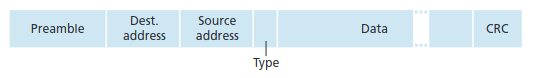
\includegraphics[width=\linewidth]{../images/w11n1ethernetFrame.png}\\
The \textbf{preamble} is 7 bytes of alternating 1s and 0s, and is used to synchronise the receiver's clock with the sender's, and is followed by a byte of \verb|10101011| to signal the start of the frame. The \textbf{destination and source addresses} are 6 bytes each, and are the MAC addresses of the sender and receiver. The \textbf{payload} is between 46 and 1500 bytes.\\
To map an IP address to a MAC address, the \textbf{address resolution protocol (ARP)} is used. A node sends a broadcast ARP request to all nodes on the network asking for the MAC address of a specific IP address. The node with that IP address then sends a unicast ARP response to the requester with its MAC address.\\
A \textbf{switch} transparently moves frames from one interface to another based on a dynamically constructed switch table. When a switch is initialised the table is empty, then when a frame arrives at an interface, the sender MAC address is stored as being on that interface, and if no frame is received from a source after a certain period of time (the \textbf{ageing time}) the entry is deleted. Switches prevent collisions if the network is setup as a start, isolate links from each other, and can automatically disconnect faulty adaptors. Switches are plug and play, and fast, but are limitted to trees with no cycles and make ARP expensive if the network is large, while routers can handle cycles and route on multiple networks, and provide firewalls and configuration, but must be configured and are slower.
